
Due to the capacity of human vision systems for highly complex processing at very low power, many brain-inspired algorithms and architectures have been proposed to emulate the human visual cortex.~\cite{Nere2011,Chen2014,Kestur2012}. %[YiranChen UPitt, Qingriu Syracuse, NEC CNN]. 

%DSPs and Heterogenous Architectures
Digital signal processors (DSPs) have been a universally accepted alternative to general purpose CPUs for seamless multimedia processing. 
The Qualcomm Hexagon DSP instruction set architecture (ISA) contains numerous special-purpose instructions designed to accelerate key multimedia kernels such as 
sliding window filters~\cite{hexagon}. 
Heterogeniety has often been considered as a viable solution to handle the increasingly varying nature of workloads that need to be run today~\cite{micro2010}.
Texas Instruments has a heterogenous multi-core DSP targeted for real-time vision applications based on their Keystone architecture. 
To tackle the diverse field of vision many other heterogenous architectures have been proposed that take advantage of 
customized flows for regular systolic operations while
using the traditional von Neumann architecture for handling control logic and other irregular data operations. A heterogenous server architecture consisting of 
many small cores for low power and high throughput coupled with custom hardware accelerators was designed in ~\cite{Iyer2011}.
In ~\cite{HPCA2015}, the authors explored architectural heterogeniety by using customized data-flows for many vision-based applications targeted at retail, 
security, etc.

%Custom Accelerators
Most vision applications demand high throughput and 
specialized accelerators have shown to be extremely performance-friendly for computationaly intensive tasks such as 
face detecion ~\cite{violafccm}, pedestrian detection~\cite{sips2014}, object recognition~\cite{Maashri2012a} and object detection~\cite{Bae2011}. In ~\cite{micro2008}, the authors propose a benchmarking suite - VISBench (Visual, Interactive, Simulation Benchmarks) - and find that a MIMD rather than a SIMD architecture gives better performance.

%\begin{figure}[!htb]
%\centering
%\tikzsetnextfilename{hog_fps}
%\begin{tikzpicture}
%\begin{axis}[
%    ybar,    
%    bar width=10pt,
%    enlarge x limits=0.1,
%    legend style={at={(0.5,-0.15)},
%    anchor=north,legend columns=-1},
%    ylabel={Frames per Second},
%    ymin = 0,
%    ymax = 40,
%    xtick=data,
%    %ytick=data,
%    symbolic x coords={0, 720x576, 1280x720, 1440x1080, 1920x1080, 5},
%    %nodes near coords,
%    %nodes near coords align={vertical},
%    ]
%\addplot [style={fill=rred}] coordinates {(720x576,15.63) (1280x720,11.76) (1440x1080,6.67) (1920x1080,4.9)};
%\addplot [style={fill=mygreen}] coordinates {(720x576,21.74) (1280x720,18.18) (1440x1080,14.49) (1920x1080,12.34)};
%\addplot [royalblue,line legend, sharp plot, update limits=false] coordinates {(0,30) (5,30)};
%\legend{CPU,GPU, Real-time}
%\end{axis}
%\end{tikzpicture}
%\caption{Frames per second}
%\label{fig:hog_fps}
%\end{figure}
With increasing image resolutions, achieving real-time performance for vision applications is becoming exceedingly difficult. 
As an example, we ran the multi-threaded Haar face detection algorithm from the latest 
stable release of OpenCV (2.4.11)~\cite{OpenCV} using 
a general purpose CPU (8 Core, Intel i7-4770 3.40 GHz,32 GB RAM, 60W) and compared the performance 
for different image resolutions.
%with a Nvidia GeForce GTX590 GPU (1024 Cuda Cores, 3GB DDR5, 300 GBps, 365W). 
Figure~\ref{fig:face_fps} shows a comparison of the two across different image sizes.
As can be seen, performance deteriorates by more than 80\% when moving from VGA to an HD image on the CPU.
Figure~\ref{fig:opencv_face_detection} shows the faces detected when the algorithm was run on an image 
from the popular PASCAL Visual Object Classes (VOC) Challenge dataset~\cite{Everingham2010}.

\begin{figure}[!htb]
\centering
\tikzsetnextfilename{face_fps}
\begin{tikzpicture}
\begin{axis}[
    ybar,    
    bar width=10pt,
    enlarge x limits=0.1,
    legend style={at={(0.5,-0.15)},
    anchor=north,legend columns=-1},
    ylabel={Frames per Second},
    ymin = 0,
    ymax = 40,
    xtick=data,
    %ytick=data,
    symbolic x coords={0, 640x480, 720x576, 1280x720, 1920x1080, 5},
    %nodes near coords,
    %nodes near coords align={vertical},
    ]
\addplot [style={fill=rred}] coordinates {(640x480,11.76) (720x576,9.43) (1280x720,4.54) (1920x1080,1.99)};
\addplot [style={fill=mygreen}] coordinates {(640x480,13) (720x576,7.4) (1280x720,3.16) (1920x1080,1.37)};
\addplot [royalblue,line legend, sharp plot, update limits=false] coordinates {(0,30) (5,30)};
\legend{Face,Person, Real-time}
\end{axis}
\end{tikzpicture}
\caption{Frames per second for face (red) and person (green) detections. Scale factor of 1.1 was used for face detection and 1.05 for person detection.}
\label{fig:face_fps}
\end{figure}

%Face Detection
\begin{figure}[htb!]
\vspace{0pt}
\centering
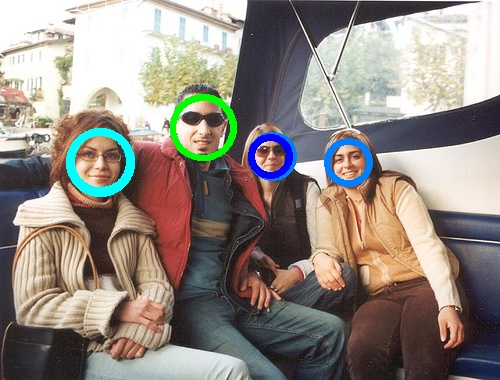
\includegraphics[width=0.9\linewidth]{./figures/facedetected.jpg}
\vspace{0pt}
\caption{Face detection algorithm results on an image from PASCAL dataset.}\label{fig:opencv_face_detection}
\vspace{0pt}
\end{figure}

%CNNs
Even though Convolutional Neural Networks (CNNs) were explored in the early 1990s for vision applications~\cite{giles1997}, they have resurfaced again after a long hiatus and become extremely popular in the past couple of years. 
This successful comeback can be attributed to two major phenomena:
(1) the existence of large amount of data (needed to train the network well) with the evolution of the digital era, and (2) the development of 
custom hardware (required for acceleration) now being used for CNNs. 

In the ImageNet Large Scale Visual Recognition Challenge (ILSVRC)
conducted in 2012, the winning team trained a CNN consisting of five convolutional and three fully-connected layers. Importantly, the depth of the CNN is critical to 
its recognition capabilities since the authors found that removing any convolutional layer resulted in inferior performance~\cite{NIPS2012}. This CNN would need
more than 80 million operations and over 100,000 data transfers~\cite{XilinxCNN}.

More recent and advanced CNN architectures have 10 to 20 layers of Rectified Linear Units, hundreds of millions of weights, and billions of connections between units.
The reader is pointed to ~\cite{Bengio2009} for insights on deep architectures in general and ~\cite{DNNNature2015} for CNN-based learning and their recent advances. 

From a systems perspective, ~\cite{Farabet2009} mapped an earlier Convolutional Network based face-detection task onto custom hardware. More recently, ~\cite{Chen2014} recently proposed an architecture for CNNs and Deep 
Neural Networks (DNNs) that minimized memory transfers thus achieving high
throughput with small area, power and energy footprint. ~\cite{DaDianNao} furthered this by proposing a training and inference accelerator 
capable of providing GPU-like bandwidth in ASIC-like power budgets.
